\newgeometry{top=1cm, bottom=2cm}
\section{Eigenwertproblem}
\begin{figure}[h!]
    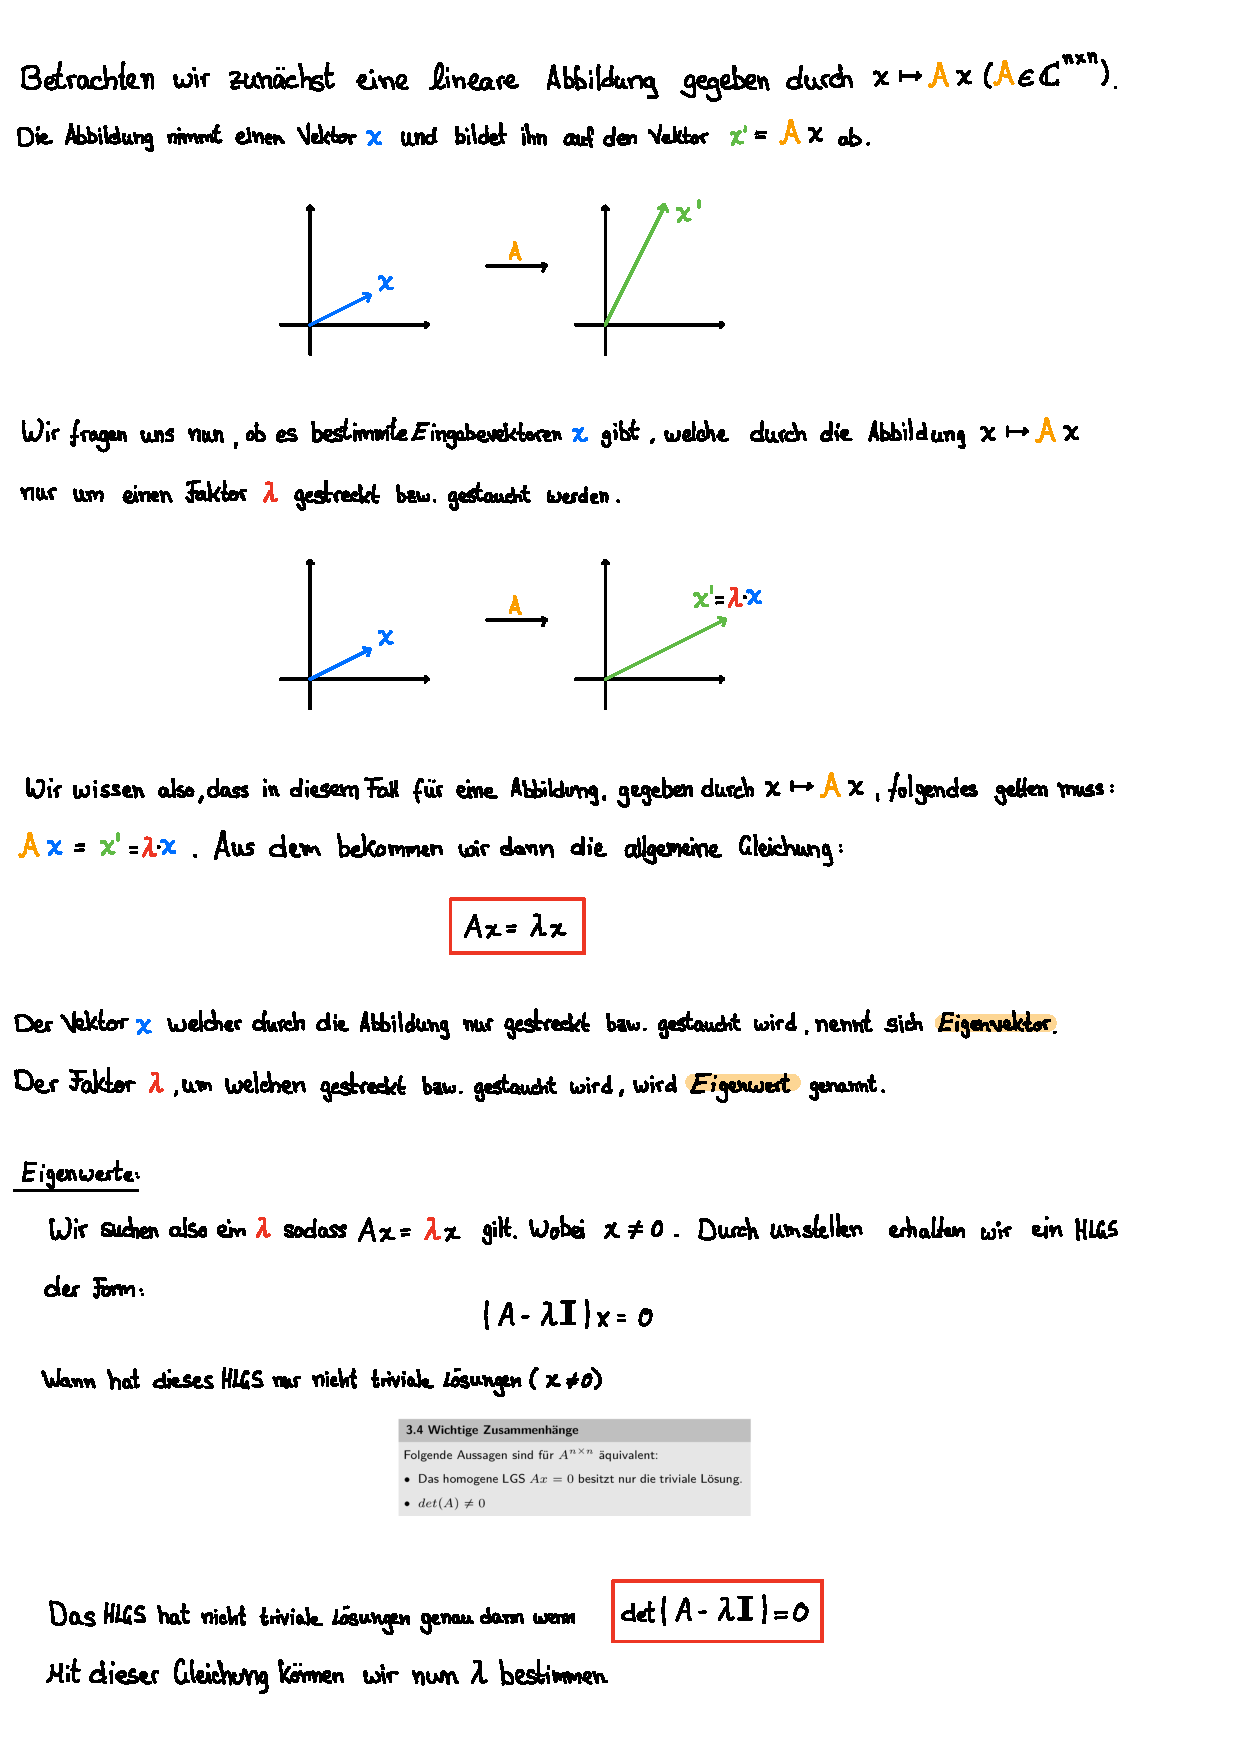
\includegraphics[page=1, scale=0.842]{pdf/06_Eigenwertproblem.pdf}
\end{figure}
\newpage
\includepdf[pages={2-}, 
            pagecommand={\thispagestyle{plain}}, 
            scale=0.95]{pdf/06_Eigenwertproblem.pdf}

\newgeometry{top=2.5cm, bottom=2cm}
\subsection{Beispielaufgaben} 
\vspace{1cm}
\subsubsection{} %Zardini S.93
Sei \[
A = \begin{pmatrix}
-3 & 4 & -4 \\
0 & 5 & -8 \\
0 & 4 & -7 \\
\end{pmatrix}.
\]
Bestimmen Sie die Eigenwerte und Eigenvektoren von $A$ und geben Sie die geometrischen und algebraischen Vielfachheiten an. \\

\noindent \textbf{Lösung:}

\newpage
\subsubsection{} %Zardini S.96
Sei \[
A = \begin{pmatrix}
-3 & 4 & -4 \\
0 & 5 & -8 \\
0 & 4 & -7 \\
\end{pmatrix}.
\]
\begin{enumerate}[label=\alph*)]
    \item Berechnen Sie das charakteristische Polynom von $A$ und überprüfen Sie ob $A$ diagonalisierbar ist.
    \item Falls möglich, diagonalisieren Sie $A$, so dass \[ D = T^{-1}AT\]
    \item Kann $T$ orthogonal gewählt werden? Falls ja, geben Sie ein solches $T$ an.
\end{enumerate}

\noindent \textbf{Lösung:}

\newpage
\subsubsection{} %Zardini S. 107
Sei \[
A = \begin{pmatrix}
5 & -6 \\
3 & -4 \\
\end{pmatrix}.
\]
Berechnen Sie $e^A$.\\

\noindent \textit{Tipp}: Das Matrixexponential vereinfacht sich für diagonalisierbare Matrizen als 
\[e^A = \sum_{n=0}^{\infty} \frac{A^n}{n!} = Tdiag(e^{\lambda_1}, ..., e^{\lambda_n})T^{-1}.\]

\noindent \textbf{Lösung:}

\newpage
\subsubsection{} %Zardini S. 110
Sei die quadratische Form $q$ gegeben durch 
\[\begin{aligned}
q: \; \mathbb{R}^2 &\rightarrow \mathbb{R} \\
q(x) &\mapsto \frac{1}{2}x_1^2 + \sqrt{3}x_1x_2-\frac{1}{2}x_2^2 \;, \;x= \begin{pmatrix}
x_1 \\
x_2\\
\end{pmatrix}
\end{aligned}\]
\begin{enumerate}[label=\alph*)]
    \item Bestimmen Sie eine symmetrische Matrix $A$, so dass $q(x)=x^\top Ax$.
    \item Führen Sie die Hauptsachentransformation $y=Tx$ durch und geben Sie die Normalform von $q$ an.
\end{enumerate}
\noindent \textbf{Lösung:}